
\section{Susceptibility calculations}
    \label{Sec:ResD:SubsceptibilityCalculation}

To verify that we do get enhanced susceptibility, leading to a spin-density wave state, the $q$-dependant susceptibility -- described in section \ref{Sec:Theo:Susceptibility} -- was calculated. Since the Lindhard function takes the sum over all energies in the Brillouin zone, there may be some concern that the rather crude adjustments to the DFT calculations performed in the previous section -- which have only been verified to be correct for energies at the Fermi surface -- may give erroneous results. However the nature of the Lindhard function means that far greater weight is given to energies that are near the Fermi surface and so, assuming that the energy dispersion does vary smoothly close to the Fermi level, any differences away from the Fermi level should not be a cause for concern.
\begin{figure}[htbp]
    \begin{center}
        \includegraphics[scale=0.9]{Chapter-dHvABaFe2P2/Figures/AngleDepMeasurements/ShiftedBandStructure/ShiftedBandStructure}
        \caption{Band structure for the bands that cross the fermi surface shifted to fit the dHvA data. (a) and (b) give an idea of the granularity of the \WIEN calculation at the Fermi surface. Inset shows the path around the brillouin zone.}
        \label{Fig:ResD:ShiftedBandStructure}
    \end{center}
\end{figure}
Calculations were performed using the \code{calc_x0.m} code described in section\ref{Sec:Exp:Susceptibility} using a $93\times93\times93$ grid of energy values that covered the first Brillouin zone. We will need to smooth over the granularity of the \WIEN band model since for the imaginary part at least, the calculations is very sensitive to slight imperfections in cancellation. Figure~\ref{Fig:ResD:ShiftedBandStructure} shows the band structure shifted as described in the previous section. We notice that away from the Fermi surface we have dicontinuities in the large hole pocket, most notably between $Z$ and $\Sigma_1$, due to the correction applied which is proprtional to the \DzTwo character however these are reasonably far from the Fermi level. Two regions in the figure are marked (a) and (b) which show points around the Fermi level as they are spaced in the $93\times93\times93$ model. (a) is particularly steep and has a $\Delta \epsilon/\textrm{pt.} = \unit[0.0760]{eV}$ and (b) is more typical of the gradient at the Fermi level and has $\Delta \epsilon/\textrm{pt.} = \unit[0.0368]{eV}$. So the energy scale that will need to compensated is \unit[$\sim 2--5\ten{-3}$]{Ry}.
\begin{figure}[htbp]
    \begin{center}
        \includegraphics[scale=0.9]{Chapter-dHvABaFe2P2/Figures/Susceptibility/RangeDeltaOmega/RangeDeltaOmega}
        \caption{Qualitative plots of the real and imaginary part of the Lindhard susceptibility calculated at $k_z=\pi$ for $T=\unit[157]{K}$ and a range of $\delta$ and $\omega$ values.}
        \label{Fig:ResD:RangeDeltaOmega}
    \end{center}
\end{figure}
Susceptibility was calculated for a wide range of magnitudes of $\delta$ and $\omega$ in order to find suitable values and qualitative plots are shown in  figure~\ref{Fig:ResD:RangeDeltaOmega}. Both the real and imaginary parts undergo qualitative changes as the parameters are adjusted above the spacing correpsonding to the typical gap in energy between points. The imaginary part also undergoes a qualitative change when $\omega$ falls below \unit[1\ten{-5}]{Ry} and there is also an increase in noise when $\delta$ falls below a similar energy threshold. We continue using $\delta=1\ten{-3}$ and $\omega=1\ten{-3}$ which correspond approximately the the energy scale of the spacing as well as the energy scale of the temperature smearing.
\begin{figure}[htbp]
    \begin{center}
        \includegraphics[scale=0.9]{Chapter-dHvABaFe2P2/Figures/Susceptibility/2DSusceptibility/2DSusceptibilityPlusAltKz}
        \caption{Real and imaginary part of the Lindhard susceptibility are plotted on the left and right respectively. Upper panels are at $k_z=\pi$ and lower are at $k_z=0$. For these calcualtions $\delta=1\ten{-3}$, $\omega=1\ten{-3}$ and $T=\unit[157.88]{K}$. Insets show contour plots for the respective surface plots.}
        \label{Fig:ResD:2DSusceptibility}
    \end{center}
\end{figure}
The upper panel of figure~\ref{Fig:ResD:2DSusceptibility} shows the quantified plots for the real and imaginary parts of the susceptibility at the chosen values of $\delta$ and $\omega$. The contour plots in the insets show the two-fold symmetry due to the choice of $k_z=\pi$. Unlike LaFeAsOF where the two dimensional approximation is a good one, this is not necessarily the case for \BaFeP which features a strongly three-dimensional hole band and some warping of the electron bands. The lower panels present the same calculation performed at $k_z=0$ which shows little change other than a rotation of the susceptibility bias due to the screw symmetry of the electron bands.
\begin{figure}[htbp]
    \begin{center}
        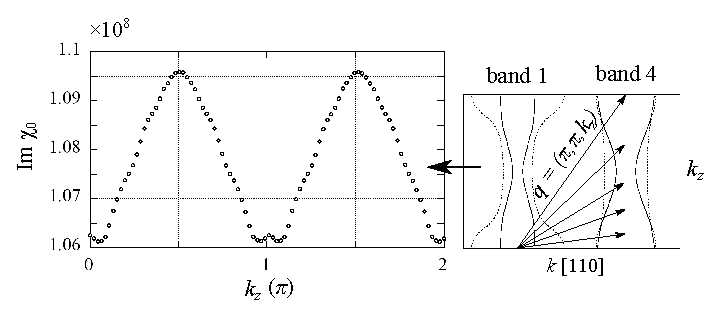
\includegraphics[scale=0.9]{Chapter-dHvABaFe2P2/Figures/Susceptibility/NestingVector/NestingVector}
        \caption{Left panel shows the real part of the Lindhard susceptibility between bands $1$ and $4$ for $q=(\pi, \pi, k_z)$ over the height of the \ac{BZ}. Peaks at $k_z=\pi/2$ and $k_z=3\pi/2$ can clearly be seen.}
        \label{Fig:ResD:NestingVector}
    \end{center}
\end{figure}
To verify that there is indeed a nesting condition at $q=(\pi, \pi, \pi/2)$ we expect to see an enhancement of the susceptibility at this $q$ vector between bands 1 and 4. Figure~\ref{Fig:ResD:NestingVector} presents the real part of the susceptibility calculated over a number of nesting vectors $q=(\pi, \pi, k_z)$ and we can see that there is indeed a moderate enhancement of around $3.2\%$ at $k_z=\pi/2, 3\pi/2$.
